% arara: pdflatex
% arara: makeglossaries
% arara: biber
% arara: pdflatex
% arara: pdflatex

\documentclass{report}

\usepackage[T1]{fontenc}%Required for special character like < and |
\usepackage{biblatex}%Reguired for "biber" to print the bibliography
\usepackage{lipsum}%Required to be able to print "Lorem ipsum"-texts
\usepackage{titlesec}%Reguired to be able for format headings.
\usepackage[hidelinks]{hyperref}%Required for links to make references and table-of-content-entries "clickable"
\usepackage[pdftex]{graphicx}%Required for graphics
\usepackage{float}%Required for example for the "H"-formatting of graphics
\usepackage{array}%Required for \newcommand{\thickhline}
\usepackage[acronym]{glossaries}%Required for glossaries
\usepackage{xcolor}%Required for \color
\usepackage{listings}%Required for listings
\usepackage{csquotes}%Required for \enquote{...}

%set title of table-of-contents
\renewcommand{\contentsname}{i18nInhaltsverzeichnis}

%import bibliography-file
\addbibresource{bibliography.bib}

%hide "Chapter X" at the beginning of chapters
\titleformat{\chapter}{\normalfont\huge\bfseries}{\thechapter}{1em}{}

%define \thickline (for tables):
\makeatletter
\newcommand{\thickhline}{
    \noalign {\ifnum 0=`}\fi \hrule height 1pt
    \futurelet \reserved@a \@xhline
}
\newcolumntype{"}{@{\hskip\tabcolsep\vrule width 1pt\hskip\tabcolsep}}
\makeatother

%hide heading of "List of tables":
\makeatletter
\renewcommand\listoftables{
    \@starttoc{lot}
}
\makeatother

%hide heading of "List of figures":
\makeatletter
\renewcommand\listoffigures{
    \@starttoc{lof}
}
\makeatother

%define glossaries:
\makeglossaries

%add dots in list for glossaries and acronyms
\renewcommand*\glspostdescription{\dotfill}

%hide heading of "Glossary"
\renewcommand{\glossarysection}[2][]{}

%glossary-entries:
\newglossaryentry{gls_entry1}{name=entry1,
  description={Description for entry1}
}
\newglossaryentry{gls_entry2}{name=entry2,
  description={Description for entry2}
}

%abbreviations:
\newacronym{acr_entry1}{XAML}{
  Extended Application Markup Language
}
\newacronym{acr_entry2}{VB}{
  Visual Basic
}

\begin{document}


%hide pagenumber on the first page
\thispagestyle{empty}
Titlepage

\newpage

\tableofcontents
\newpage

\chapter{i18nAbstract}
abstracttext

\chapter{Examples}
\section{Special character}
example: \textbackslash \textasciitilde \\
a<b>c|d/'`¿ÇäöüÄÖÜßé@!23\\
this is some \enquote{quoted text}.

\section{Figures}
A figure:
\begin{figure}[H]
    \centering
    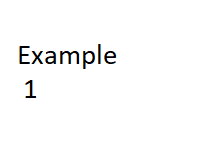
\includegraphics{figures/examples/test1.png}
    \caption{Figure 1 caption}\label{fig:fig1}
\end{figure}
another figure:
\begin{figure}[H]
    \centering
    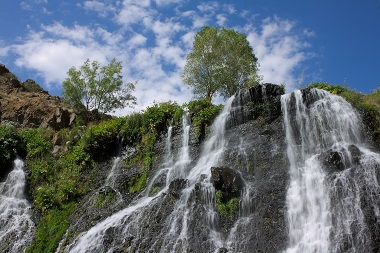
\includegraphics{figures/examples/test2.jpg}
    \caption{Figure 2 caption}\label{fig:fig2}
\end{figure}

\section{Lists}
itemize:
\begin{itemize}
    \item This is an entry
    \item This is another entry
\end{itemize}
enumerate:
\begin{enumerate}
    \item This is an entry
    \item This is another entry
\end{enumerate}

\section{Tables}
A table:
\begin{table}[H]
    \centering
    \begin{tabular}{ | l | c | r | }\hline
        1 & 2 & 3 \\\hline
        4 & 5 & 6 \\\hline
        7 & 8 & 9 \\\hline
    \end{tabular}
    \caption{Table 1 caption}\label{tab:tab1}
\end{table}
Another table:
\begin{table}[H]
    \centering
    \begin{tabular}{ | l | c | r | }\hline
        1 & 2 & 3 \\\thickhline
        4 & 5 & 6 \\\hline
        7 & 8 & 9 \\\hline
    \end{tabular}
    \caption{Table 2 caption}\label{tab:tab2}
\end{table}

\section{References}\label{sec:ref}
This sentence has a reference to a bibliography-item (article).\cite{ein1}\\
This sentence also has a reference to a bibliography-item (book).\cite{gam1}\\
This sentence also has a reference to a bibliography-item (online).\cite{sho1}\\
This sentence has a simple footnote.\footnote{some footnote-text}\\
This is the usage of a glossary-entry: \gls{gls_entry1}\\
This is the usage of another glossary-entry: \gls{gls_entry2}\\
This is the first usage of an acronym: \gls{acr_entry1}\\
This is the first usage of another acronym: \gls{acr_entry2}\\
This is the seconds usage of an acronym: \gls{acr_entry1}\\
This is the seconds usage of another acronym: \gls{acr_entry2}\\
This is a reference to figure1: \ref{fig:fig1}\\
This is a reference to table1: \ref{tab:tab2}\\
This is a reference to section \ref{sec:ref}\\

\section{Listings}
Some listing defined in an file:
\lstinputlisting[backgroundcolor = \color{lightgray},caption={listing 1}]{listing1.py}
some other listing from another file:
\lstinputlisting[backgroundcolor = \color{lightgray},caption={listing 2}]{listing2.py}

\chapter{Einführung}
\lipsum

\chapter{Analyse}
\lipsum

\chapter{Fazit}
\lipsum

\chapter{i18nVerzeichnisse}

\section{i18nAbbildungsverzeichnis}
\listoffigures
\newpage

\section{i18nTabellenverzeichnis}
\listoftables
\newpage

\section{i18nAbkürzungsverzeichnis}
\printacronyms
\newpage

\section{i18nGlossar}
\printglossary
\newpage

\section{i18nLiteraturverzeichnis}
\printbibliography[heading=none]

\chapter{i18nAnhang}
\section{Anhang1}
some anhang
\section{Anhang2}
some anhang
\section{Anhang3}
some anhang

\chapter{i18nSelbstständigkeitserklärung}
some text

\end{document}
